% =========================================================
% SECTION: TEXT DATA EDA
% =========================================================
\section{Exploratory Data Analysis: Text Data}
\label{sec:text}

\subsection{Dataset Overview}
For the text modality, we used the \textbf{SMS Spam Collection Dataset}, a well-known benchmark for binary text classification in natural language processing research. The dataset consists of English-language SMS messages labeled as either \texttt{ham} (legitimate personal messages) or \texttt{spam} (unsolicited promotional messages).

\begin{itemize}
    \item \textbf{Source:} \href{https://www.kaggle.com/datasets/marslinoedward/sms-spam-dataset/data}{SMS Spam Dataset --- Kaggle (marslinoedward)}
\end{itemize}

\begin{importantbox}
\textbf{Dataset Statistics:}
\begin{itemize}
    \item \textbf{Total Messages:} 5{,}572
    \item \textbf{Unique Messages:} 5{,}169 \hfill (403 exact duplicate rows detected)
    \item \textbf{Features:} 2 columns --- \texttt{label} (categorical: ham/spam) and \texttt{text} (raw string)
    \item \textbf{Ham (legitimate):} 4{,}825 messages \quad \textbf{86.6\%}
    \item \textbf{Spam:} 747 messages \quad \textbf{13.4\%}
    \item \textbf{Missing values:} 0 --- all rows are complete
\end{itemize}
\end{importantbox}

The class distribution is visualised in the figure below. The dataset contains approximately 6.5 ham messages for every 1 spam message --- a realistic ratio reflecting real-world SMS traffic, but one that has important implications for modelling: a naive majority-class classifier that always predicts ``ham'' achieves \textbf{86.6\% accuracy without learning anything}. Standard accuracy is therefore a misleading evaluation metric; F1-score (macro or weighted), Precision, Recall, and AUC-ROC are more appropriate.

\begin{figure}[H]
    \centering
    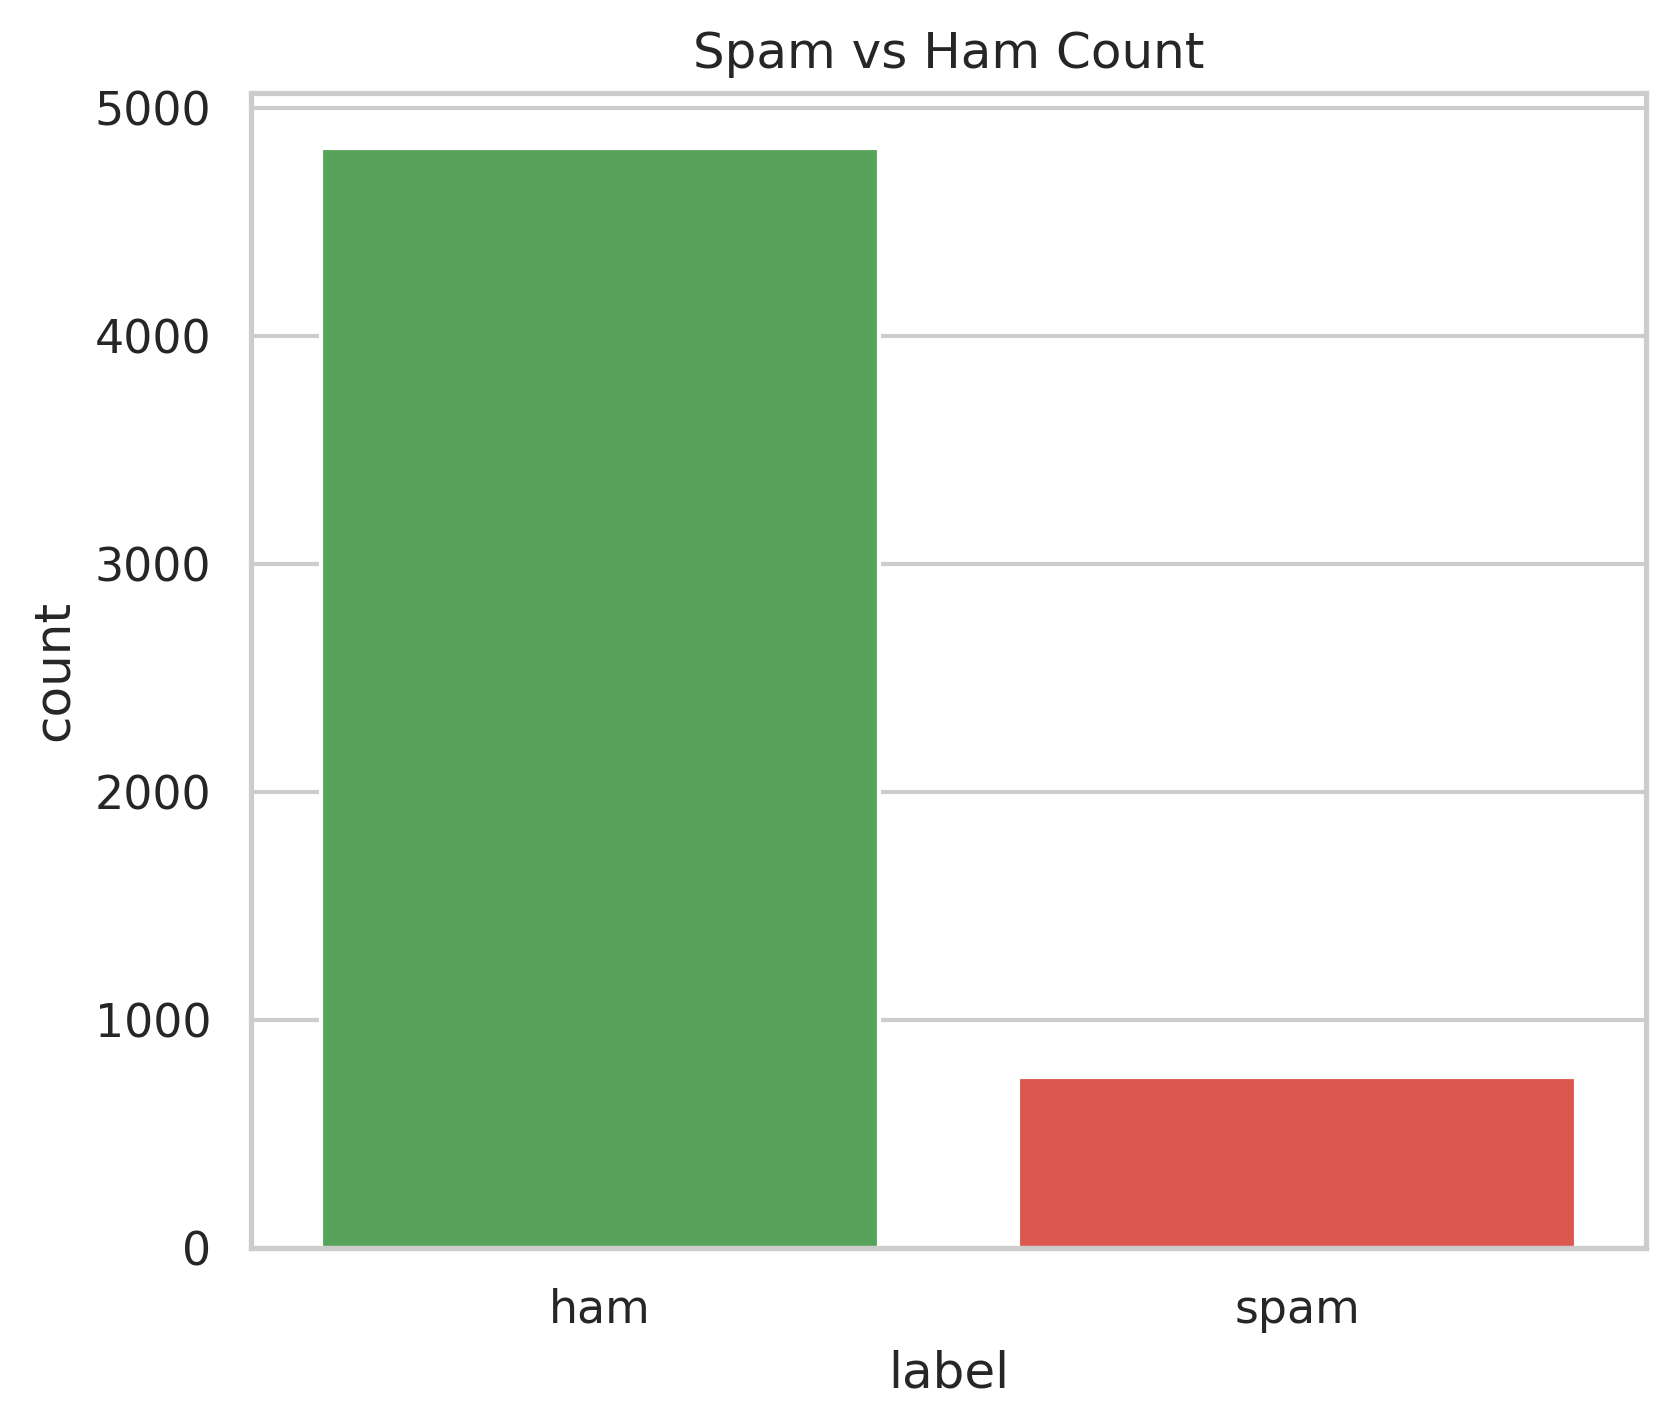
\includegraphics[width=0.60\textwidth]{images/text_target_dist.png}
    \caption{\textbf{Figure T1} --- Class Distribution: Ham vs.\ Spam (5{,}572 total messages; 86.6\%:13.4\%).
    \textit{Code:} \texttt{df\_text['label'].value\_counts().plot(kind='bar')}.}
    \label{fig:text_target}
\end{figure}

\subsection{Data Inspection and Quality}

\begin{itemize}
    \item \textbf{Shape:} \texttt{(5572, 2)} --- 5{,}572 rows, 2 columns (\texttt{label}, \texttt{text}).
    \item \textbf{Missing values:} None. Every row has both a label and a non-empty text field, making the dataset immediately usable without imputation.
    \item \textbf{Duplicate messages:} 403 exact duplicate rows detected (\texttt{df.duplicated().sum()}). These are predominantly very short, common ham phrases (``Ok'', ``I'll call you later'') that naturally recur across different conversation threads. While they do not represent data corruption, duplicates can introduce \emph{data leakage} if the same message appears in both train and test splits. \textbf{Deduplication is recommended} before any train/test split.
    \item \textbf{Label encoding:} \texttt{ham} $\rightarrow$ 0, \texttt{spam} $\rightarrow$ 1 for modelling.
\end{itemize}

\subsection{Message Length Analysis}

Message character length is one of the simplest yet most powerful raw features for separating ham from spam. Table T1 below summarises the statistics by label, and the resulting distributions are shown in Figure T2.

\begin{table}[H]
\centering
\caption{\textbf{Table T1} --- Message Length Statistics by Label (character count, including spaces)}
\label{tab:text_length}
\begin{tabular}{lrrrr}
\hline
\textbf{Label} & \textbf{Mean} & \textbf{Median} & \textbf{Min} & \textbf{Max} \\
\hline
Ham  & $\sim$71.5  & 52  & 2   & 910 \\
Spam & $\sim$138.7 & 149 & 13  & 224 \\
\hline
\end{tabular}
\end{table}

Key observations:
\begin{itemize}
    \item \textbf{Spam is nearly twice as long:} Mean spam length ($\sim$139 chars) is almost double that of ham ($\sim$72 chars). Spam authors pack promotional content, phone numbers, URLs, and urgency cues into each message.
    \item \textbf{Spam is length-bounded:} Maximum spam length (224 chars) is well below maximum ham length (910 chars), reflecting spammers' optimization for the 160-character SMS limit while legitimate messages can span multiple segments.
    \item \textbf{Low variance in spam:} Spam messages cluster tightly around the median (median $\approx$ mean $\approx$ 149 chars), indicating templated, length-optimised message structures.
    \item \textbf{High variance in ham:} Ham shows a long right tail (max = 910), ranging from single-word replies (``Ok'') to detailed multi-paragraph personal messages.
\end{itemize}

\begin{figure}[H]
    \centering
    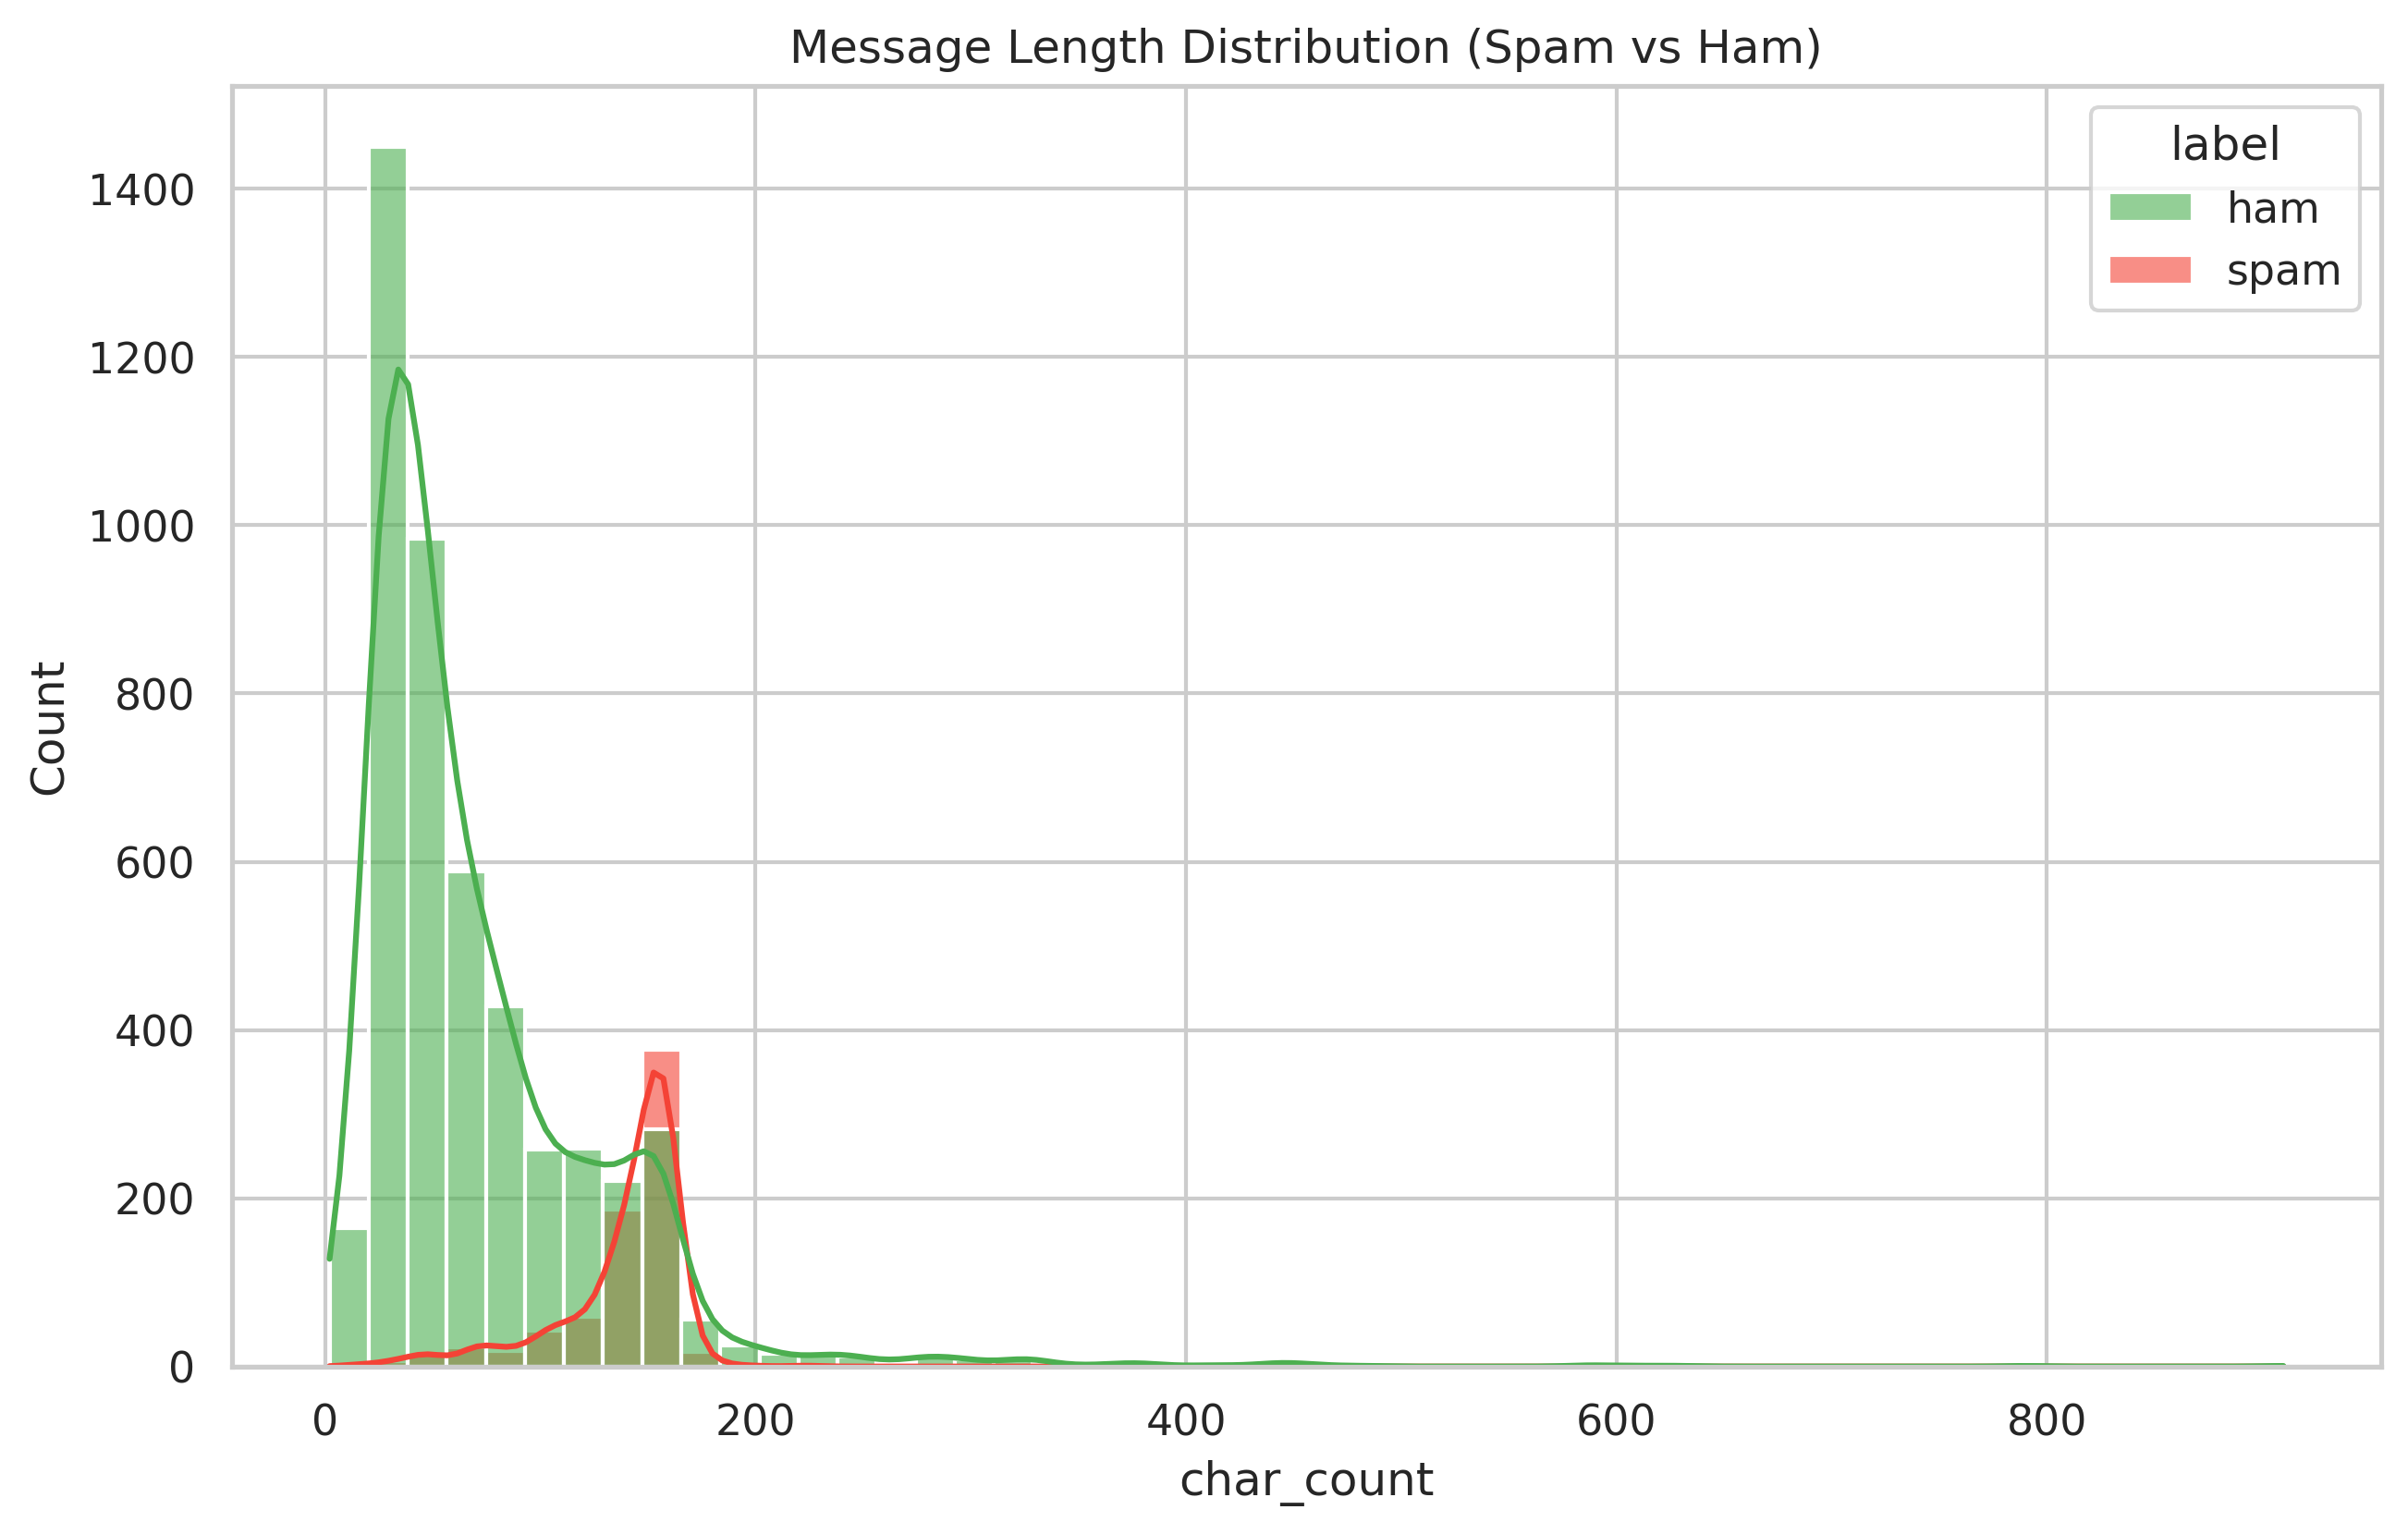
\includegraphics[width=0.92\textwidth]{images/msg_length_dist.png}
    \caption{\textbf{Figure T2} --- Message Length Distribution: Histogram (left) and Boxplot (right) comparing Ham vs.\ Spam.
    \textit{Code:} \texttt{df['length'] = df['text'].apply(len)}, then \texttt{plt.hist()} and \texttt{df.boxplot(column='length', by='label')}.}
    \label{fig:text_length}
\end{figure}

\subsection{Vocabulary and Word Cloud Analysis}

Word clouds (Figure T3 below) were generated using the \texttt{WordCloud} library on each label's concatenated text. The visual contrast is immediately striking:

\begin{itemize}
    \item \textbf{Ham (green):} Dominated by everyday conversational words --- \textit{call}, \textit{come}, \textit{going}, \textit{time}, \textit{day}, \textit{know}, \textit{will}. These reflect the informal, relational nature of legitimate SMS exchanges.
    \item \textbf{Spam (red):} Dominated by promotional language --- \textit{free}, \textit{win}, \textit{prize}, \textit{claim}, \textit{txt}, \textit{urgent}, \textit{call}. Notably, ``call'' appears in both corpora but in fundamentally different contexts: personal calls in ham vs.\ calls to premium-rate numbers in spam.
\end{itemize}

\begin{figure}[H]
    \centering
    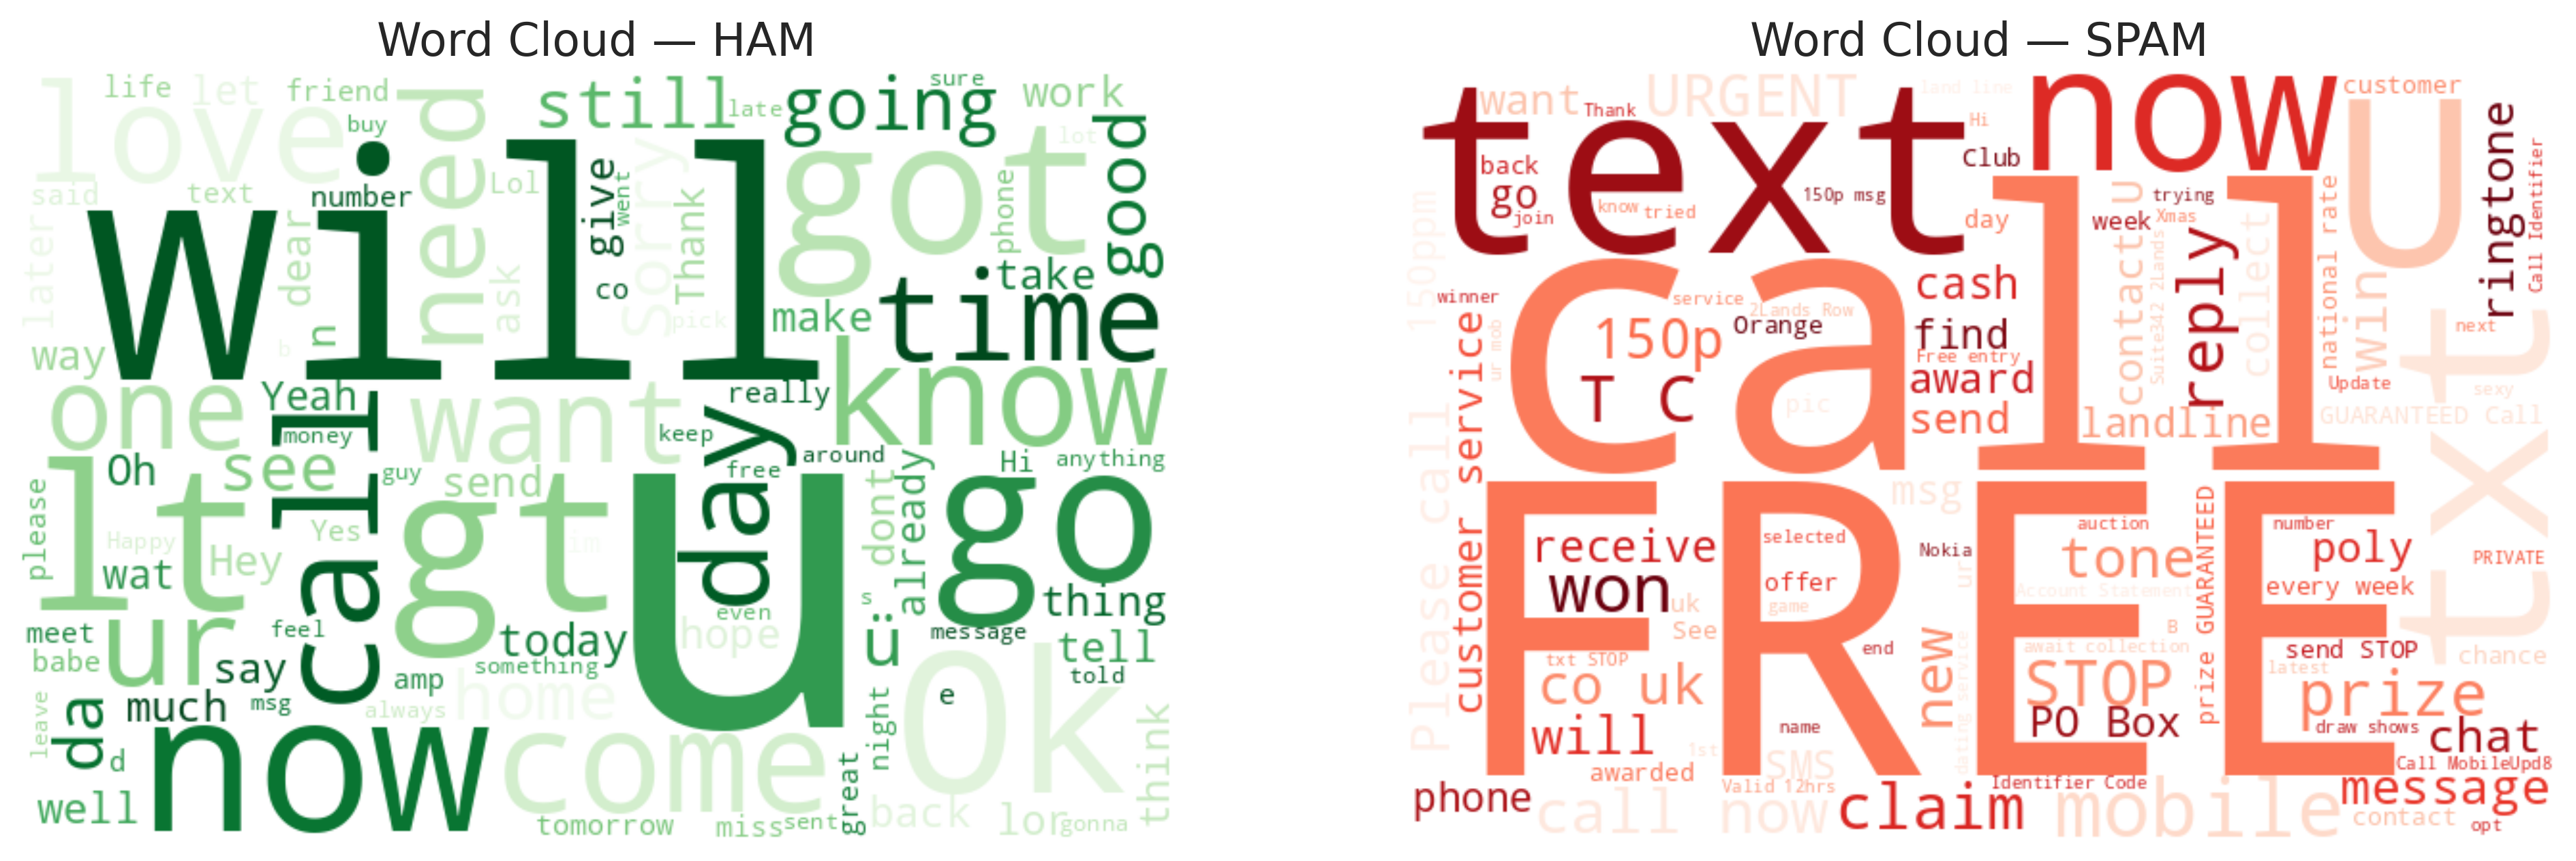
\includegraphics[width=0.90\textwidth]{images/wordclouds.png}
    \caption{\textbf{Figure T3} --- Word Clouds for Ham (left, green) and Spam (right, red).
    \textit{Code:} \texttt{WordCloud(max\_words=200, background\_color='white').generate(text)} per label.}
    \label{fig:wordclouds}
\end{figure}

\subsection{Token Frequency Analysis}

\subsubsection*{Step 1 --- Top Overall Tokens (Before Preprocessing)}

Figure T4 below shows the 20 most frequent tokens across the full corpus before any preprocessing. The list is dominated by high-frequency function words (``I'', ``to'', ``a'', ``u'', ``you'') that carry no discriminative power between classes. This motivates the stopword removal step.

\begin{figure}[H]
    \centering
    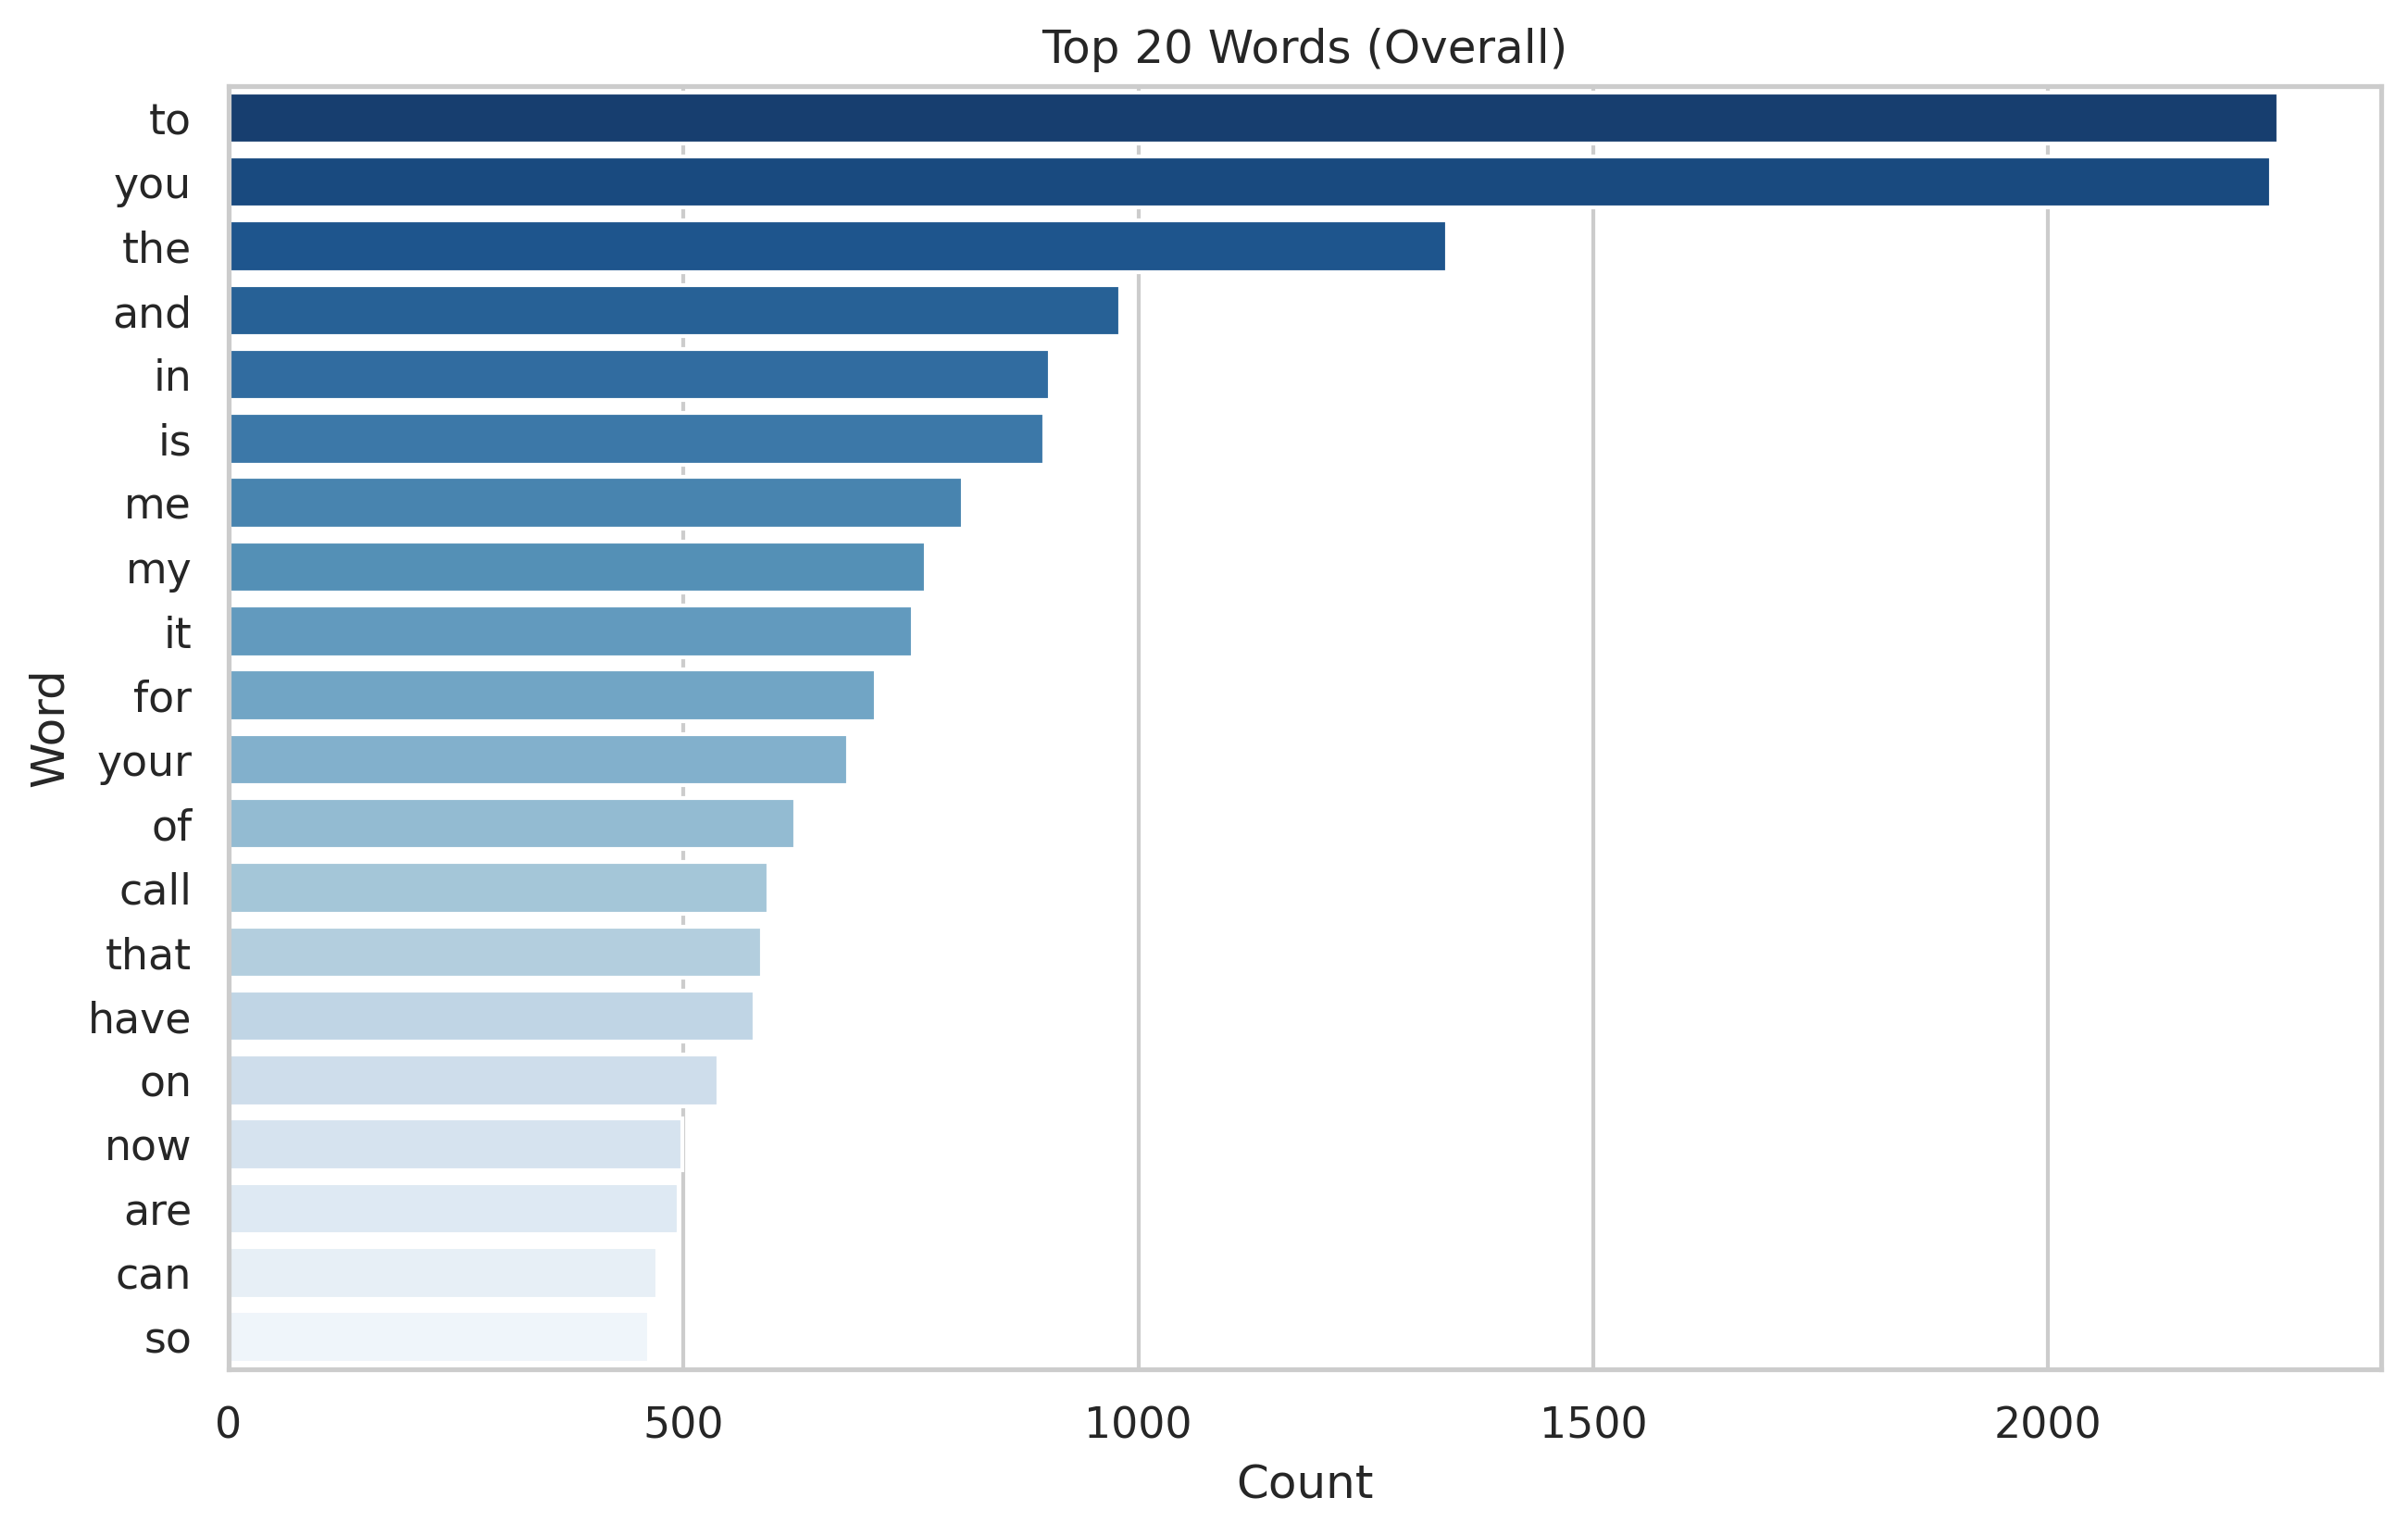
\includegraphics[width=0.85\textwidth]{images/top_overall.png}
    \caption{\textbf{Figure T4} --- Top 20 Most Frequent Tokens across the Full Corpus (stopwords included).
    \textit{Code:} \texttt{Counter(all\_tokens).most\_common(20)}.}
    \label{fig:text_top_overall}
\end{figure}

\subsubsection*{Step 2 --- Identifying Stopwords}

Figure T5 below isolates the top stopwords found in the corpus. Their dominance in the raw frequency list confirms that stopword removal is a necessary preprocessing step.

\begin{figure}[H]
    \centering
    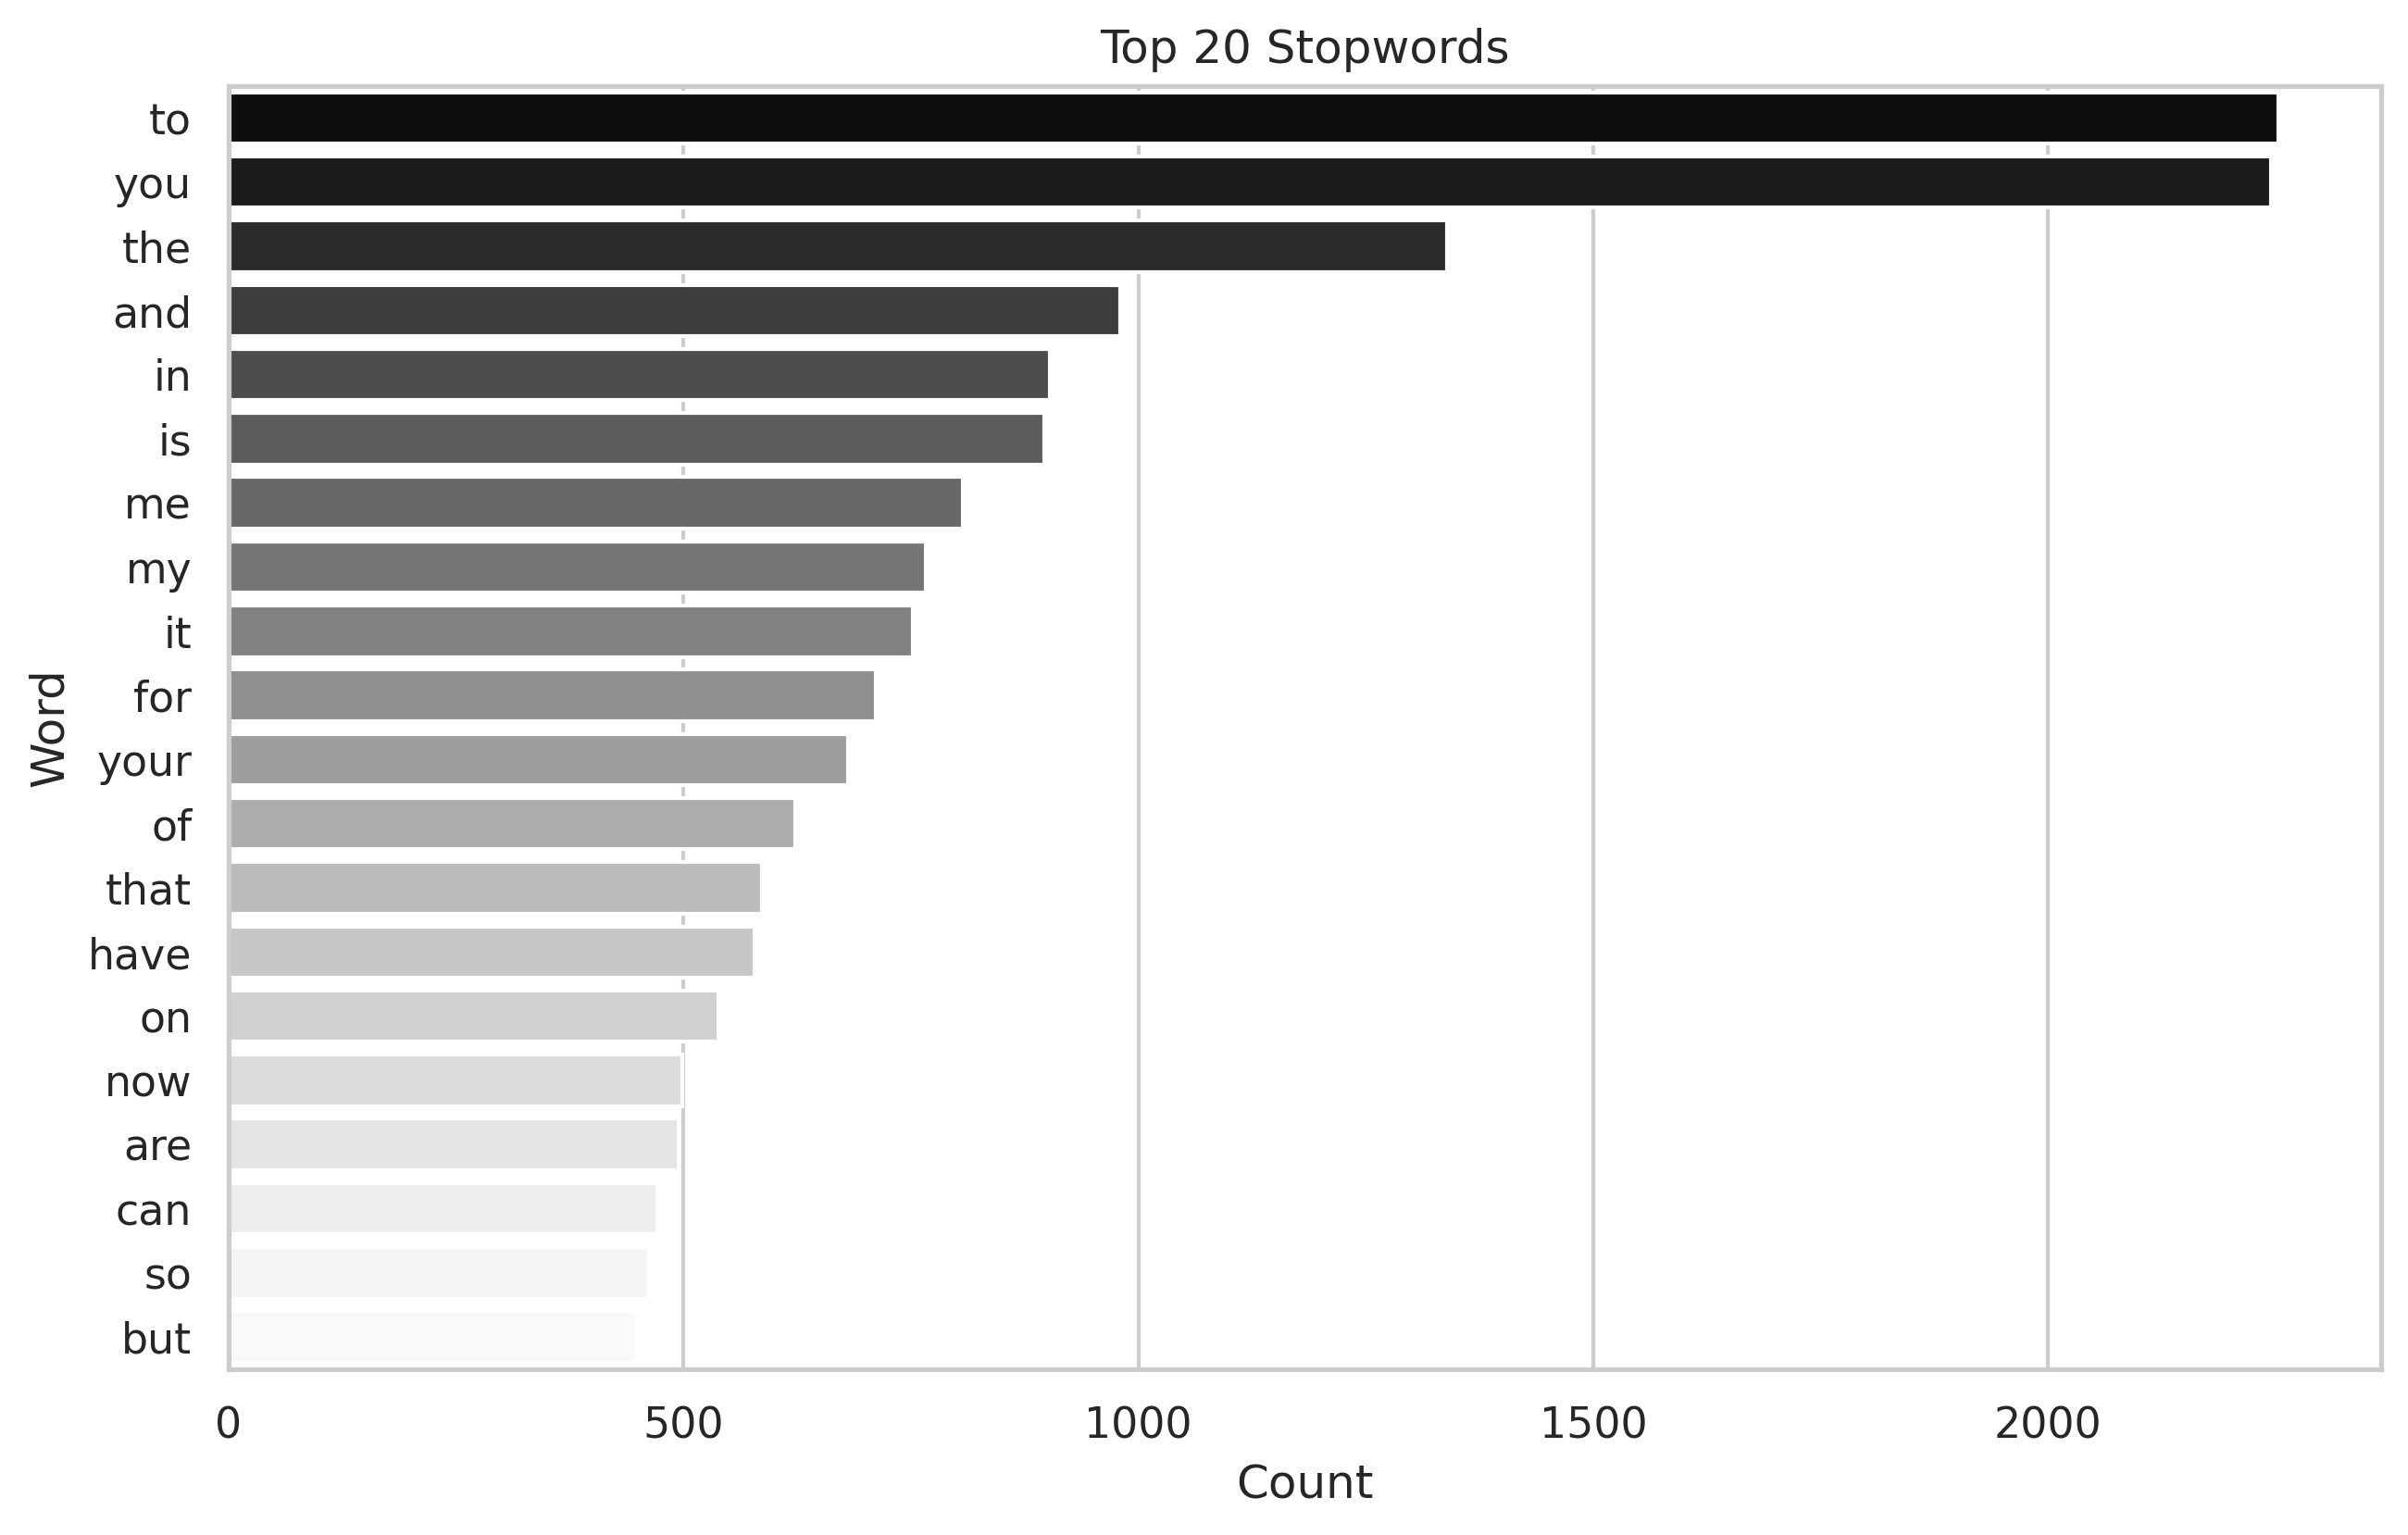
\includegraphics[width=0.85\textwidth]{images/top_stopwords.png}
    \caption{\textbf{Figure T5} --- Top Stopwords in the Corpus. Removing these exposes the discriminative vocabulary.
    \textit{Code:} Frequency count on a curated stopword set intersected with all tokens.}
    \label{fig:text_top_stopwords}
\end{figure}

\subsubsection*{Step 3 --- Top Discriminative Tokens (After Stopword Removal)}

Figure T6 below shows the class-specific top tokens after removing standard English stopwords. The class separation is clear:

\begin{itemize}
    \item \textbf{Spam-associated:} \textit{free}, \textit{win}, \textit{prize}, \textit{claim}, \textit{txt}, \textit{mobile} --- promotional, action-driving vocabulary.
    \item \textbf{Ham-associated:} \textit{call}, \textit{come}, \textit{good}, \textit{time}, \textit{day}, \textit{know} --- natural everyday conversational terms.
\end{itemize}

\begin{figure}[H]
    \centering
    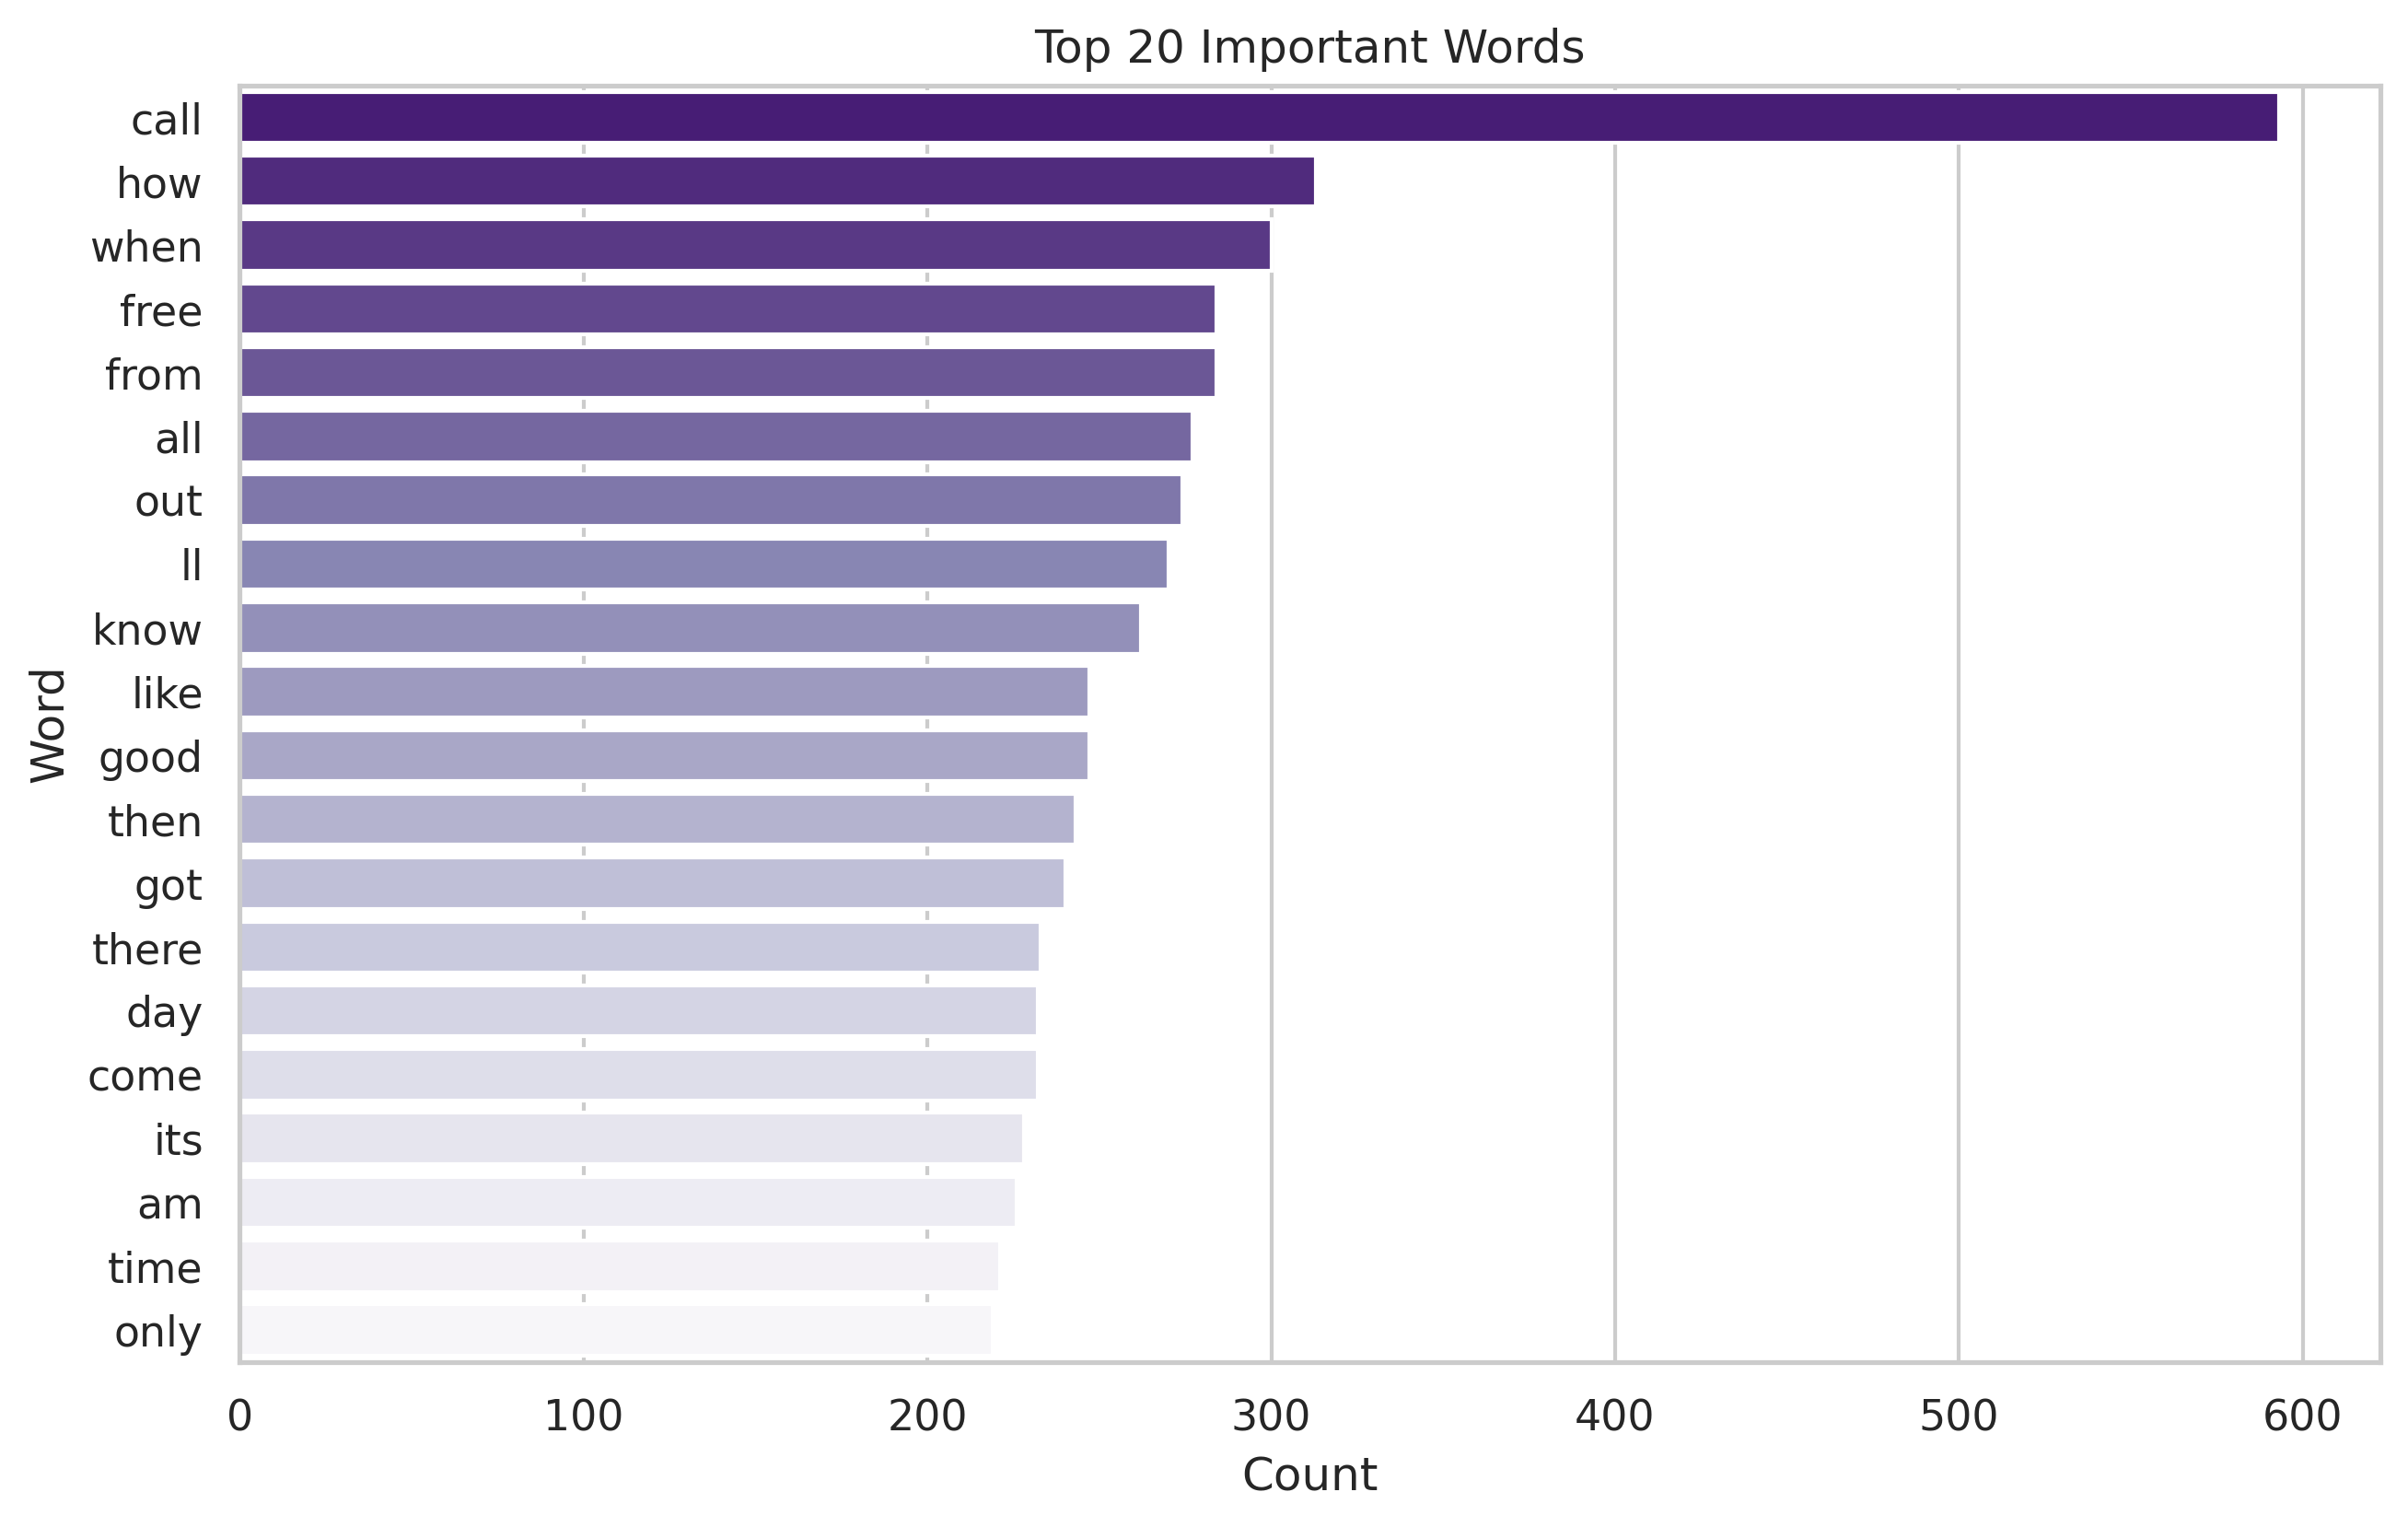
\includegraphics[width=0.85\textwidth]{images/top_important.png}
    \caption{\textbf{Figure T6} --- Top Discriminative Tokens After Stopword Removal, split by class (ham vs.\ spam).
    \textit{Code:} \texttt{Counter(filtered\_tokens).most\_common(15)} per label subset.}
    \label{fig:text_top_important}
\end{figure}

\subsection{N-gram Analysis}

Single-token frequencies miss multi-word patterns. Figure T7 below extends the analysis to bigrams and trigrams, revealing formulaic phrase patterns unique to each class:

\begin{itemize}
    \item \textbf{Spam bigrams / trigrams:} ``free entry'', ``text to win'', ``win a prize'', ``call now'', ``cash prize'' --- short promotional formulas that function as near-perfect spam signatures.
    \item \textbf{Ham bigrams / trigrams:} ``going to'', ``can I'', ``let me know'', ``talk to you'' --- natural conversational connectors typical of personal SMS dialogue.
\end{itemize}

N-gram features (e.g., a TF-IDF vectoriser with \texttt{ngram\_range=(1,2)}) are expected to be highly informative for this classification task, outperforming unigram-only approaches.

\begin{figure}[H]
    \centering
    
\includegraphics[width=0.95\textwidth]{images/top_bigrams.png}
    \caption{\textbf{Figure T7} --- Bigram and Trigram Frequency Analysis by Label (Ham vs.\ Spam).
    \textit{Code:} \texttt{Counter(ngrams(tokens, n)).most\_common(12)} per label, displayed with \texttt{ax.barh()}.}
    \label{fig:text_bigrams}
\end{figure}

\subsection{Word Count vs.\ Character Count}

Figure T8 below scatterplots the word count (number of whitespace-delimited tokens) against character count for each message, coloured by label. The two classes form visually separable clusters:

\begin{itemize}
    \item \textbf{Ham cluster:} Dispersed cloud at low-to-moderate word and character counts, with a long tail of very long messages (the multi-segment personal messages reaching 910 chars).
    \item \textbf{Spam cluster:} Compact, dense region at moderate-to-high word counts and moderate character counts (roughly 100--224 chars), consistent with templated messages optimised for the 160-char SMS limit.
\end{itemize}

The visual separation confirms that \textbf{both word count and character count are strong discriminating features} even without any NLP preprocessing.

\begin{figure}[H]
    \centering
    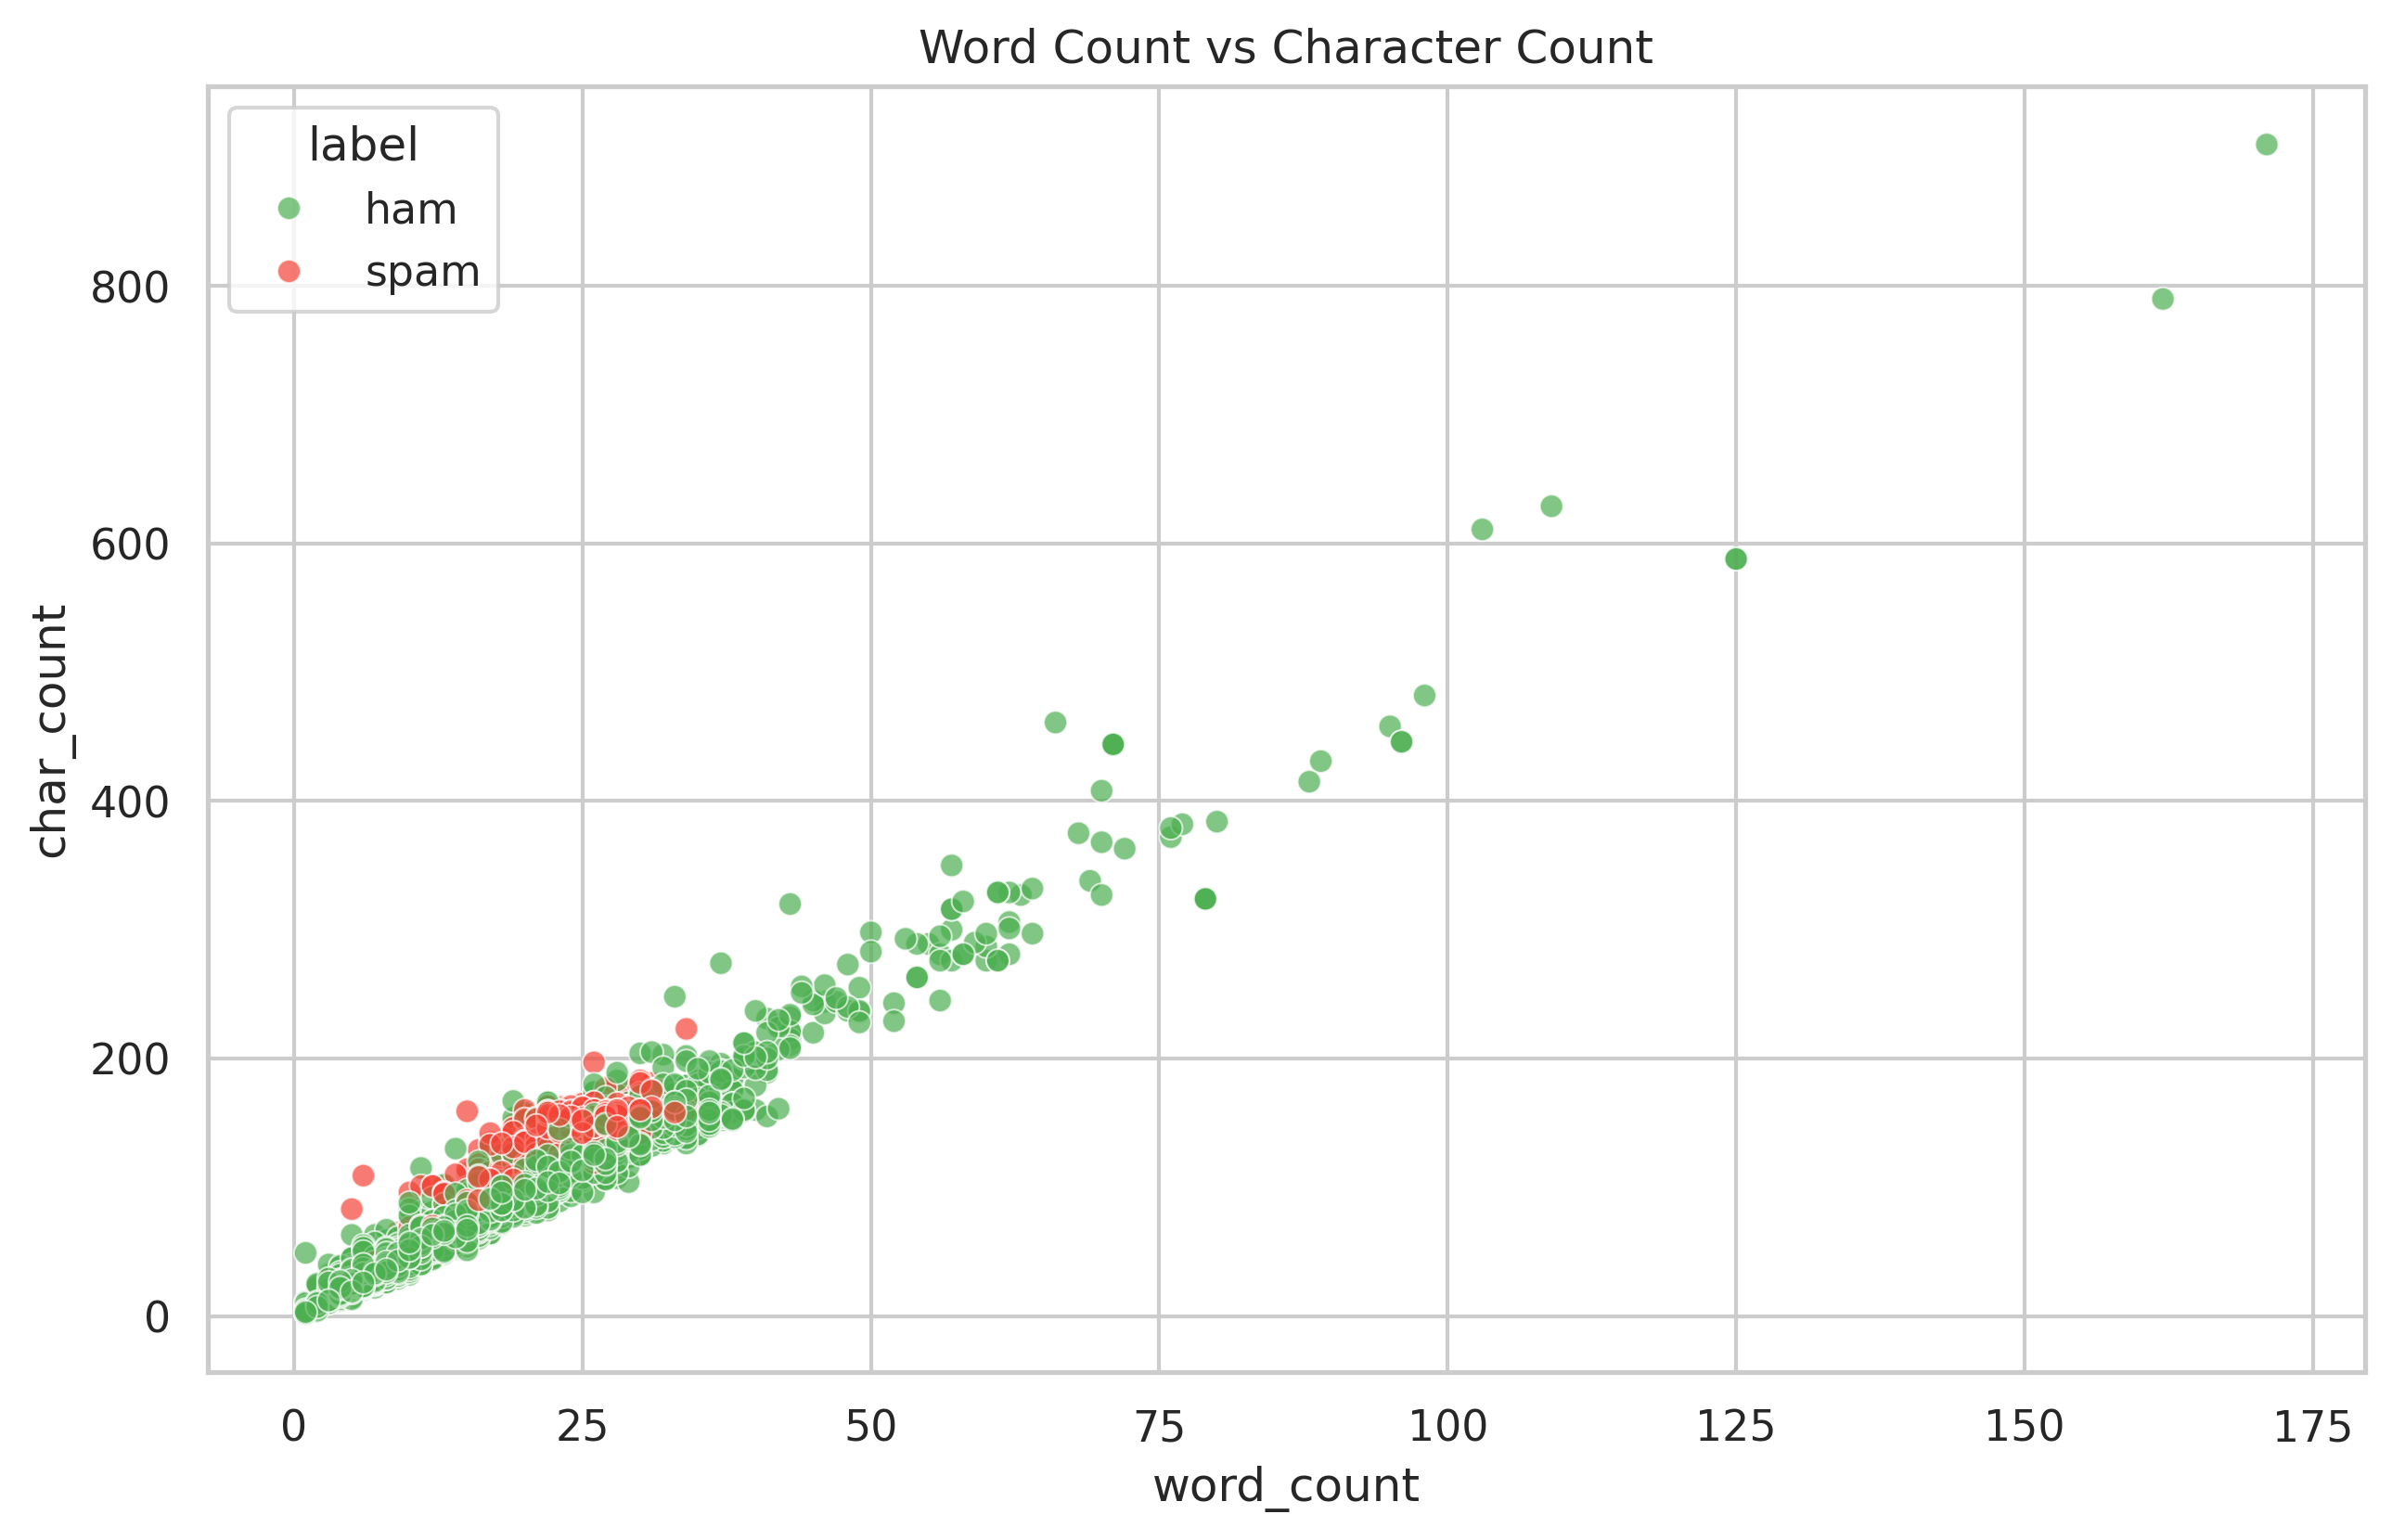
\includegraphics[width=0.75\textwidth]{images/word_vs_char.png}
    \caption{\textbf{Figure T8} --- Word Count vs.\ Character Count per message, coloured by label.
    \textit{Code:} \texttt{df['n\_words'] = df['text'].str.split().str.len()}, then \texttt{plt.scatter()}.}
    \label{fig:text_word_vs_char}
\end{figure}

% ---------------------------------------------------------
\subsection{Special Character and URL Feature Analysis}

Beyond raw length and vocabulary, \textbf{structural features} of the message text reveal strong spam signals. The following six binary or ratio features were engineered and compared between classes:

\begin{itemize}
    \item \textbf{Upper Ratio:} Fraction of characters that are uppercase.
    \item \textbf{Exclamation:} Number of \texttt{!} characters per message.
    \item \textbf{Dollar:} Number of \texttt{\$} characters per message.
    \item \textbf{Has URL:} 1 if the message contains \texttt{http}, \texttt{www}, or \texttt{.com}; else 0.
    \item \textbf{Has Phone:} 1 if the message contains a sequence of $\geq 5$ digits (phone number); else 0.
    \item \textbf{Has Number:} 1 if any digit appears in the message; else 0.
\end{itemize}

Table T2 below summarises the mean values per class, and Figure T9 visualises each feature side-by-side:

\begin{table}[H]
\centering
\caption{\textbf{Table T2} --- Mean Special Feature Values by Label}
\label{tab:text_features}
\begin{tabular}{lrr}
\hline
\textbf{Feature} & \textbf{Ham} & \textbf{Spam} \\
\hline
Upper Ratio  & 0.059 & 0.111 \\
Exclamation  & 0.177 & 0.730 \\
Dollar (\$)  & 0.000 & 0.000 \\
Has URL      & 0.004 & 0.162 \\
Has Phone    & 0.001 & 0.756 \\
Has Number   & 0.157 & 0.948 \\
\hline
\end{tabular}
\end{table}

\begin{figure}[H]
    \centering
    
\includegraphics[width=0.95\textwidth]{images/text_features.png}
    \caption{\textbf{Figure T9} --- Special Feature Comparison: Ham (green) vs.\ Spam (red) for 6 engineered features. Bar height = mean value across all messages in that class.
    \textit{Code:} Feature engineering via regex and \texttt{str.count()}, then \texttt{groupby('label').mean()} and \texttt{plt.bar()}.}
    \label{fig:text_features}
\end{figure}

Key observations from Figure T9:
\begin{itemize}
    \item \textbf{Has Phone is the strongest discriminator:} 75.6\% of spam contains a phone number vs.\ only 0.06\% of ham. A phone number in a message is an almost certain spam indicator.
    \item \textbf{Has Number is nearly universal in spam:} 94.8\% of spam messages contain at least one digit (prize amounts, phone numbers, competition codes) vs.\ only 15.7\% of ham.
    \item \textbf{URL presence signals spam:} 16.2\% of spam contains a URL or web address vs.\ only 0.35\% of ham. Spam links typically drive recipients to phishing or premium-rate sites.
    \item \textbf{Exclamation marks signal urgency:} Spam uses exclamation marks $4\times$ more than ham (mean 0.73 vs.\ 0.18), consistent with urgency-driven promotional language.
    \item \textbf{Uppercase emphasis:} Spam has nearly $2\times$ the uppercase ratio (0.111 vs.\ 0.059), reflecting the ``SHOUTING'' style of spam (e.g., ``WIN NOW'', ``FREE PRIZE'').
    \item \textbf{Dollar sign inconclusive:} Both classes show near-zero dollar sign usage in this dataset --- it is not a useful feature here.
\end{itemize}

% ---------------------------------------------------------
\subsection{Vocabulary Richness Analysis (Type-Token Ratio)}

The \textbf{Type-Token Ratio (TTR)} measures vocabulary richness: it is the ratio of unique words (types) to total words (tokens). A higher TTR indicates more diverse, less repetitive language.

\begin{table}[H]
\centering
\caption{\textbf{Table T3} --- Vocabulary Richness Comparison: Ham vs.\ Spam}
\label{tab:text_ttr}
\begin{tabular}{lrrr}
\hline
\textbf{Label} & \textbf{Total Words} & \textbf{Unique Words} & \textbf{TTR} \\
\hline
Ham  & 69{,}905 & 6{,}709 & 0.0960 \\
Spam & 15{,}819 & 1{,}940 & 0.1226 \\
\hline
\end{tabular}
\end{table}

Figure T10 below visualises three vocabulary richness metrics side-by-side:

\begin{figure}[H]
    \centering
    
\includegraphics[width=0.95\textwidth]{images/text_vocab_richness.png}
    \caption{\textbf{Figure T10} --- Vocabulary Richness Analysis: Unique Word Count (left), Type-Token Ratio / TTR (centre), and Average Word Length (right) for Ham vs.\ Spam.
    \textit{Code:} \texttt{len(set(tokens)) / len(tokens)} for TTR; \texttt{np.mean([len(w) for w in tokens])} for avg word length.}
    \label{fig:text_vocab_richness}
\end{figure}

Key observations from Figure T10 and Table T3 above:
\begin{itemize}
    \item \textbf{Ham has a larger raw vocabulary} (6{,}709 unique words vs.\ 1{,}940 for spam), reflecting the more open-ended, natural language of legitimate messages.
    \item \textbf{Spam has a higher TTR} (0.1226 vs.\ 0.0960) despite a smaller absolute vocabulary. This is because ham's corpus is much larger (69{,}905 tokens vs.\ 15{,}819) --- the TTR naturally decreases with corpus size as common words repeat more. The higher spam TTR reflects its \emph{smaller corpus size}, not greater vocabulary diversity.
    \item \textbf{Spam uses longer words on average} (4.97 chars/word vs.\ 4.17 for ham), likely due to promotional terms like ``congratulations'', ``guaranteed'', ``unsubscribe''.
    \item \textbf{Implication:} TTR is corpus-size dependent and should be used cautiously as a standalone feature; it is more reliable when computed on messages of equal length.
\end{itemize}

% ---------------------------------------------------------
\subsection{Key Findings}

\begin{importantbox}
\textbf{Summary of Text EDA Key Findings:}
\begin{itemize}
    \item \textbf{Class imbalance:} Ham (86.6\%) $\gg$ Spam (13.4\%). Naive accuracy is highly misleading; use F1 (macro), AUC-ROC, or Precision/Recall as primary metrics.
    \item \textbf{Length as a zero-cost feature:} Spam ($\sim$139 chars average) is nearly \textbf{2$\times$ longer} than ham ($\sim$72 chars). Message length provides strong discriminating power with zero preprocessing cost.
    \item \textbf{Structural spam signals (strongest first):}
    \begin{enumerate}
        \item Has Phone number: 75.6\% spam vs.\ 0.06\% ham (highest discriminative power)
        \item Has Number (any digit): 94.8\% spam vs.\ 15.7\% ham
        \item Has URL: 16.2\% spam vs.\ 0.35\% ham
        \item Exclamation marks: mean 0.73 spam vs.\ 0.18 ham
        \item Uppercase ratio: 11.1\% spam vs.\ 5.9\% ham
    \end{enumerate}
    \item \textbf{Vocabulary contrast:} Spam relies on promotional vocabulary (\textit{free, win, prize, claim, txt}); ham uses everyday conversational language. The vocabularies are largely non-overlapping for the most frequent class-specific terms.
    \item \textbf{N-gram signatures:} Spam contains formulaic phrase patterns (``free entry'', ``text to win'') absent from ham, making bigram TF-IDF features highly informative.
    \item \textbf{Vocabulary richness (TTR):} Ham has a larger absolute vocabulary (6{,}709 unique words); spam uses longer individual words (avg 4.97 chars/word vs.\ 4.17 for ham).
    \item \textbf{Recommended preprocessing pipeline:}
    \begin{enumerate}
        \item Lowercasing and whitespace-based tokenisation.
        \item Standard English stopword removal.
        \item Stemming or lemmatisation (Porter Stemmer / WordNet Lemmatiser).
        \item Removal of URLs, phone numbers, currency symbols, and special characters.
        \item Class balancing via SMOTE or class-weighted cross-entropy loss.
    \end{enumerate}
    \item \textbf{Recommended models:} TF-IDF + Logistic Regression or Na\"{i}ve Bayes as an interpretable baseline; fine-tuned DistilBERT for state-of-the-art performance.
\end{itemize}
\end{importantbox}
